\documentclass[10pt, colorlinks=true, urlcolor=blue]{beamer}

% Themes and colors for a professional look
\usetheme{Madrid}
\usecolortheme{seagull}
\setbeamercolor{title}{fg=white,bg=blue!80!black}
\setbeamercolor{frametitle}{fg=white,bg=blue!70!black}
\setbeamercolor{block title}{fg=white,bg=blue!80!black}
\setbeamercolor{block body}{bg=blue!5!white}
\setbeamerfont{title}{size=\fontsize{12}{16}\selectfont}
\setlength{\parindent}{0pt}

% Customize the footline layout
\setbeamertemplate{footline}
{
  \leavevmode%
  \hbox{%
    % Left field (author or custom text)
    \begin{beamercolorbox}[wd=0.25\paperwidth,ht=2.5ex,dp=1ex,center]{author in head/foot}%
      \usebeamerfont{author in head/foot}\insertshortauthor
    \end{beamercolorbox}%
    % Middle field (title)
    \begin{beamercolorbox}[wd=0.5\paperwidth,ht=2.5ex,dp=1ex,center]{title in head/foot}%
      \usebeamerfont{title in head/foot}\insertshorttitle
    \end{beamercolorbox}%
    % Right field (page number)
    \begin{beamercolorbox}[wd=0.25\paperwidth,ht=2.5ex,dp=1ex,center]{date in head/foot}%
      \usebeamerfont{date in head/foot}\insertframenumber/\inserttotalframenumber
    \end{beamercolorbox}%
  }%
}

% Set hyperlink colors
\hypersetup{
    colorlinks=true,    % Enable colored links
    urlcolor=blue,      % Color for URLs
    linkcolor=blue      % Color for internal links (optional)
}

\usepackage{minted}

\title{Memory\_Graph, a Python Teaching Tool and Debugger Aid}
\author{Bas Terwijn}
\titlegraphic{
\vspace{-2.8em} % Adjust this value as needed
  \makebox[\textwidth]{%
  \begin{tabular}{c c}
    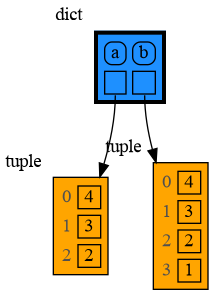
\includegraphics[height=0.35\textwidth]{figures/immutable.png} &
    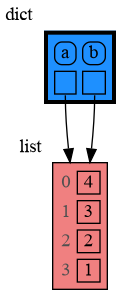
\includegraphics[height=0.35\textwidth]{figures/mutable.png} \\
      &  \\
    \multicolumn{2}{c}{
      
\includegraphics[width=0.6\textwidth]{figures/uva.png}
    }
  \end{tabular}
}
}
\date{}

\begin{document}

\begin{frame}
    \titlepage
\end{frame}

\begin{frame}{Topics}
  \begin{enumerate}
    \item Explain Python Data Model (to demo Memory\_Graph)
    \item Data Model Exercises
    \item Data Structure examples
    \item Integration in IDEs
  \end{enumerate}
\end{frame}

\begin{frame}{Python Data Mode}
  \begin{block}{Python Types}
    Python has two distinct categories of types: Immutable, Mutable
  \end{block}
  
  \vspace{2.4em}
  
  \textbf{Immutable} Types: \texttt{bool}, \texttt{int}, \texttt{float}, \texttt{complex}, \texttt{str}, \texttt{tuple}, \texttt{bytes}, \texttt{frozenset} \\
  
  \vspace{-0.8em}
  A value of an immutable type \textbf{cannot} be mutated in place. \\
  So when it is changed, \textbf{an} automatic copy is made. \\
  
  \vspace{2.0em}
  
  \textbf{Mutable} Types: \texttt{list}, \texttt{set}, \texttt{dict}, \texttt{classes}, \dots (most other types) \\
  
  \vspace{-0.8em}
  A value of a mutable type \textbf{can} be mutated in place. \\
  So when it is changed, \textbf{no} copy is made.
\end{frame}


\begin{frame}[fragile]{Mutability, live in ipython}
  \begin{minted}[fontsize=\small]{python}
  a = (4, 3, 2)  # tuple, immutable
  b = a
  b += (1,)

  c = [4, 3, 2]  # list, mutable
  d = c
  d += [1]
  \end{minted}
\end{frame}

\begin{frame}[fragile]{Copying, live in Web Debugger}
  To copy values yourself, Python has three ways:
 \href{https://memory-graph.com/#code=import+copy%0A%0Aa+%3D+%5B+%5B1%2C+2%5D%2C+%5B%27x%27%2C+%27y%27%5D+%5D%0A%0Ac1+%3D+a++++++++++++++++%0Ac2+%3D+copy.copy%28a%29+++++%0Ac3+%3D+copy.deepcopy%28a%29+%0A%0A%23+c1%3A+assignment%2C+++nothing+is+copied%2C+everything+is+shared%0A%23+c2%3A+shallow+copy%2C+first+element+is+copied%2C+underlying+is+shared%0A%23+c3%3A+deep+copy%2C++++everything+is+copied%2C+nothing+is+shared%0A}{Copying} \\
 \vspace{1em}

 Or define your own custom copy logic:
 \href{https://memory-graph.com/#code=import+copy%0A%0Aa+%3D+%5B+%5B1%2C+2%5D%2C+%5B%27x%27%2C+%27y%27%5D+%5D%0A%0Ac1+%3D+a++++++++++++++++%0Ac2+%3D+copy.copy%28a%29+++++%0Ac3+%3D+copy.deepcopy%28a%29+%0A%0A%23+c1%3A+assignment%2C+++nothing+is+copied%2C+everything+is+shared%0A%23+c2%3A+shallow+copy%2C+first+element+is+copied%2C+underlying+is+shared%0A%23+c3%3A+deep+copy%2C++++everything+is+copied%2C+nothing+is+shared%0A%0Adef+custom_copy%28a%29%3A%0A++++c+%3D+a.copy%28%29+%23+shallow+copy%0A++++c%5B1%5D+%3D+a%5B1%5D.copy%28%29%0A++++return+c%0A++++%0Ac4+%3D+custom_copy%28a%29%0A%0A%23+c4%3A+custom+copy%2C+++you+decide+what+is+copied+and+shared%0A&breakpoints=18}{Custom Copy}
\end{frame}


\begin{frame}[fragile]{Name Rebinding, live in Web Debugger}
  Difference between changing and reassigning:
  \href{https://memory-graph.com/#code=%0Aa+%3D+%5B4%2C+3%2C+2%5D%0Ab+%3D+a%0A%0Ab+%2B%3D+%5B1%5D++++++++%23+changing+%27b%27+changes+%27a%27%0Ab+%3D+%5B100%2C+200%5D++%23+but+reassignment+rebinds+%27b%27+to+another+value%2C+%27a%27+is+uneffected%0A}{Name Rebinding}
\end{frame}

\begin{frame}{Data Model Exercises}
  \href{https://memory-graph.com/#codeurl=https://raw.githubusercontent.com/bterwijn/memory_graph_videos/refs/heads/main/exercises/exercise9.py}{test}
  % \href{https://memory-graph.com/#codeurl=https://raw.githubusercontent.com/bterwijn/memory_graph_videos/refs/heads/main/exercises/exercise9.py}{Exercise 9}
  %\begin{enumerate}
  % \item \href{https://memory-graph.com/#codeurl=https://raw.githubusercontent.com/bterwijn/memory_graph_videos/refs/heads/main/exercises/exercise9.py}{Exercise 9}
  % \item \href{https://memory-graph.com/#codeurl=https://raw.githubusercontent.com/bterwijn/memory_graph_videos/refs/heads/main/exercises/exercise8.py}{Exercise 8}
  % \item \href{https://memory-graph.com/#codeurl=https://raw.githubusercontent.com/bterwijn/memory_graph_videos/refs/heads/main/exercises/exercise5.py}{Exercise 5}
  %\item test
  %\end{enumerate}


\end{frame}




\end{document}
